%
% main.tex - a typical phil presentation
%
% Copyright (c) 2015, Phil Maker
% GPLv2 
% 
%    

\documentclass{beamer}
%\documentclass[a4paper,handout]{beamer}
%\usepackage{pgfpages}
%\pgfpagesuselayout{4 on 1}[a4paper,border shrink=5mm]

\mode<presentation>{\usetheme{Pjm}}
\usepackage{graphics}
\usepackage{fancyvrb}
\newenvironment{code}
{\Verbatim[fontfamily=courier,%
numbers=right,stepnumber=5,%
firstnumber=\the\inputlineno]}%
{\endVerbatim}
\usepackage[english]{babel}
%\usepackage[latin1]{inputenc}
\usepackage{hyperref}
\definecolor{links}{HTML}{2A1B81}
\hypersetup{
  pdftitle = {Southern Exposure: an overview of PV/Diesel in
  Malaysia and Australia},
  pdfsubject = {PV Diesel}
  pdfkeywords = {Energy, Renewables, Powerwater, Phil Maker},
  pdfauthor = {\textcopyright\ Phil Maker, ...},
  pdfcreator = {\LaTeX\ with package \flqq hyperref \frqq},
  colorlinks,linkcolor=,urlcolor=links
}
\usepackage{xcolor}
\definecolor{JungleGreen}{cmyk}{0.99,0,0.52,0}
\definecolor{BlueGreen}{cmyk}{0.85,0,0.33,0}
\definecolor{RawSienna}{cmyk}{0,0.72,1,0.45}
\def\dill#1{\textcolor{RawSienna}{\textbf{Dill Alert: #1}}}

\title{Southern Exposure: an overview of PV/Diesel in Malaysia and
  Australia} 
\author{Phil Maker\\
  \href{mailto:philip.maker@gmail.com}{\texttt{<philip.maker@gmail.com>}}
}
\institute{Alaskan Center for Energy and Power}
\date{March 2015}
\logo{
\includegraphics[height=0.7cm]{logo.jpg}}
\begin{document}

\begin{frame}
  \maketitle
  \vspace{-0.6cm}
  \begin{abstract}
    \small A summary of efforts in Malaysia and Australia in the
    PV/Diesel/Battery area with Malaysia mostly winning (no comment re Alaska).
  \end{abstract}
\end{frame}

\section{Introduction}
\begin{frame}\frametitle{Introduction}
Overview of PV/Diesel/Battery work in:
 
  \begin{enumerate}
  \item Australia
  \item Malaysia
  \item Sky Cameras and Solar Forecasting
  \end{enumerate}

\pause
\vfill
\begin{quote}
``Remember that every view,
\pause
is based on where you are looking from'' -- Uncle Phil
\end{quote}

\end{frame}

\begin{frame}\frametitle{PV for 1 week}
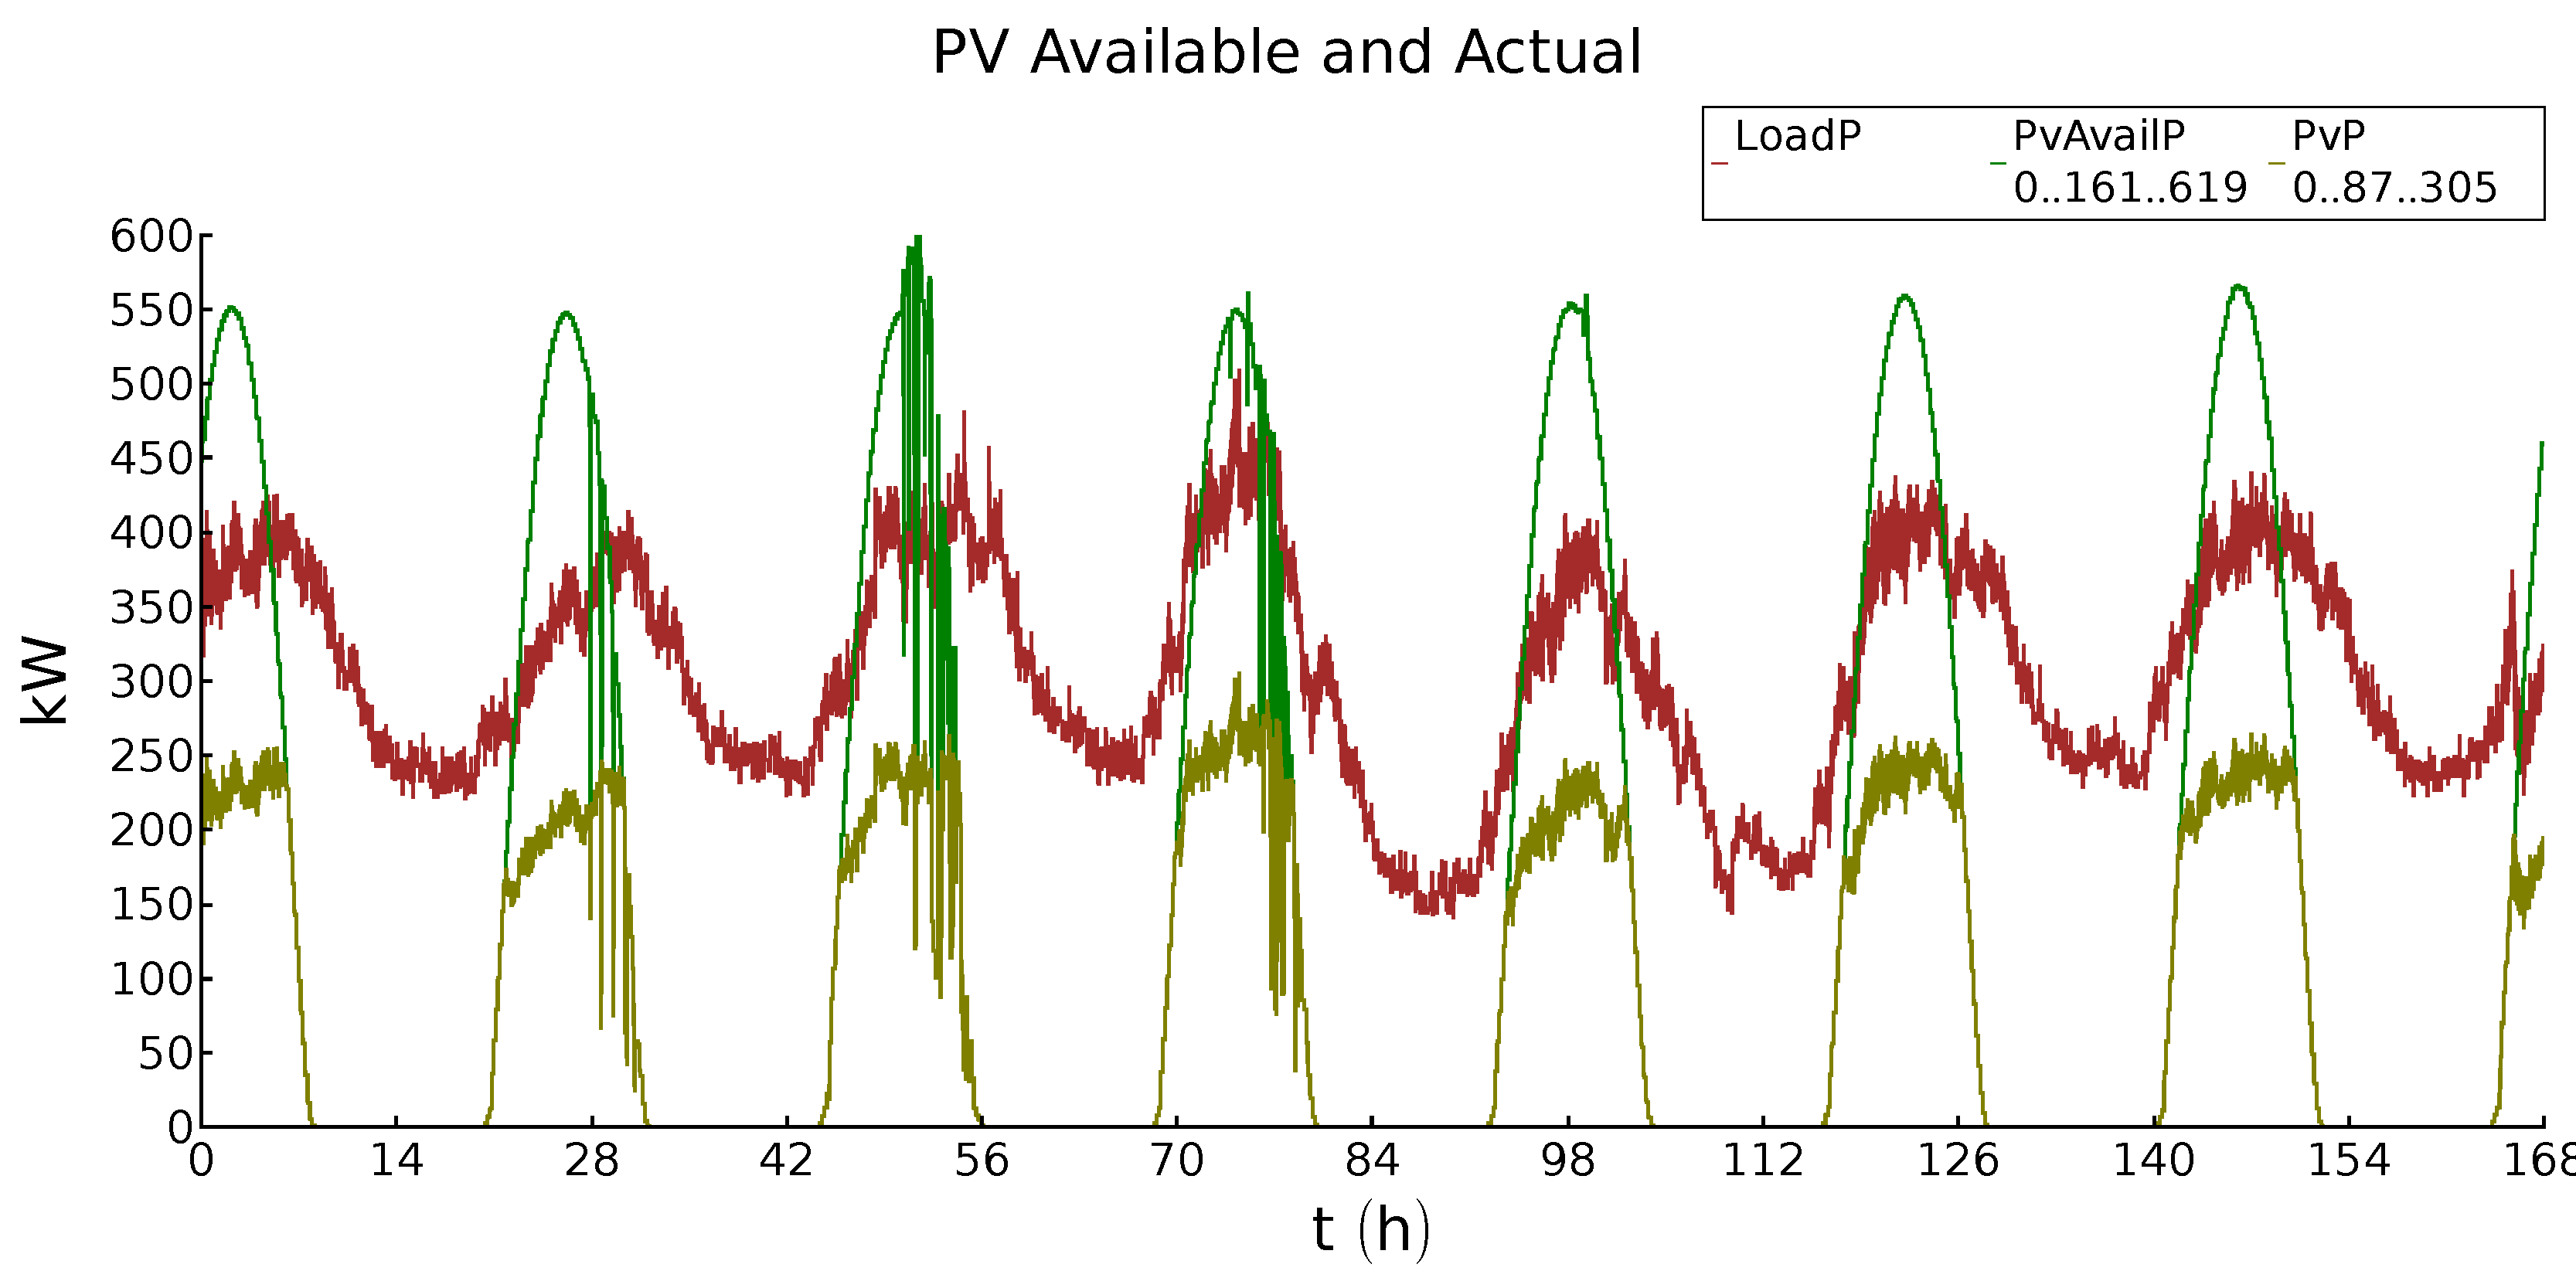
\includegraphics[width=9cm]{figPv1.pdf}  
\end{frame}

\begin{frame}\frametitle{PV variation for 1 week}
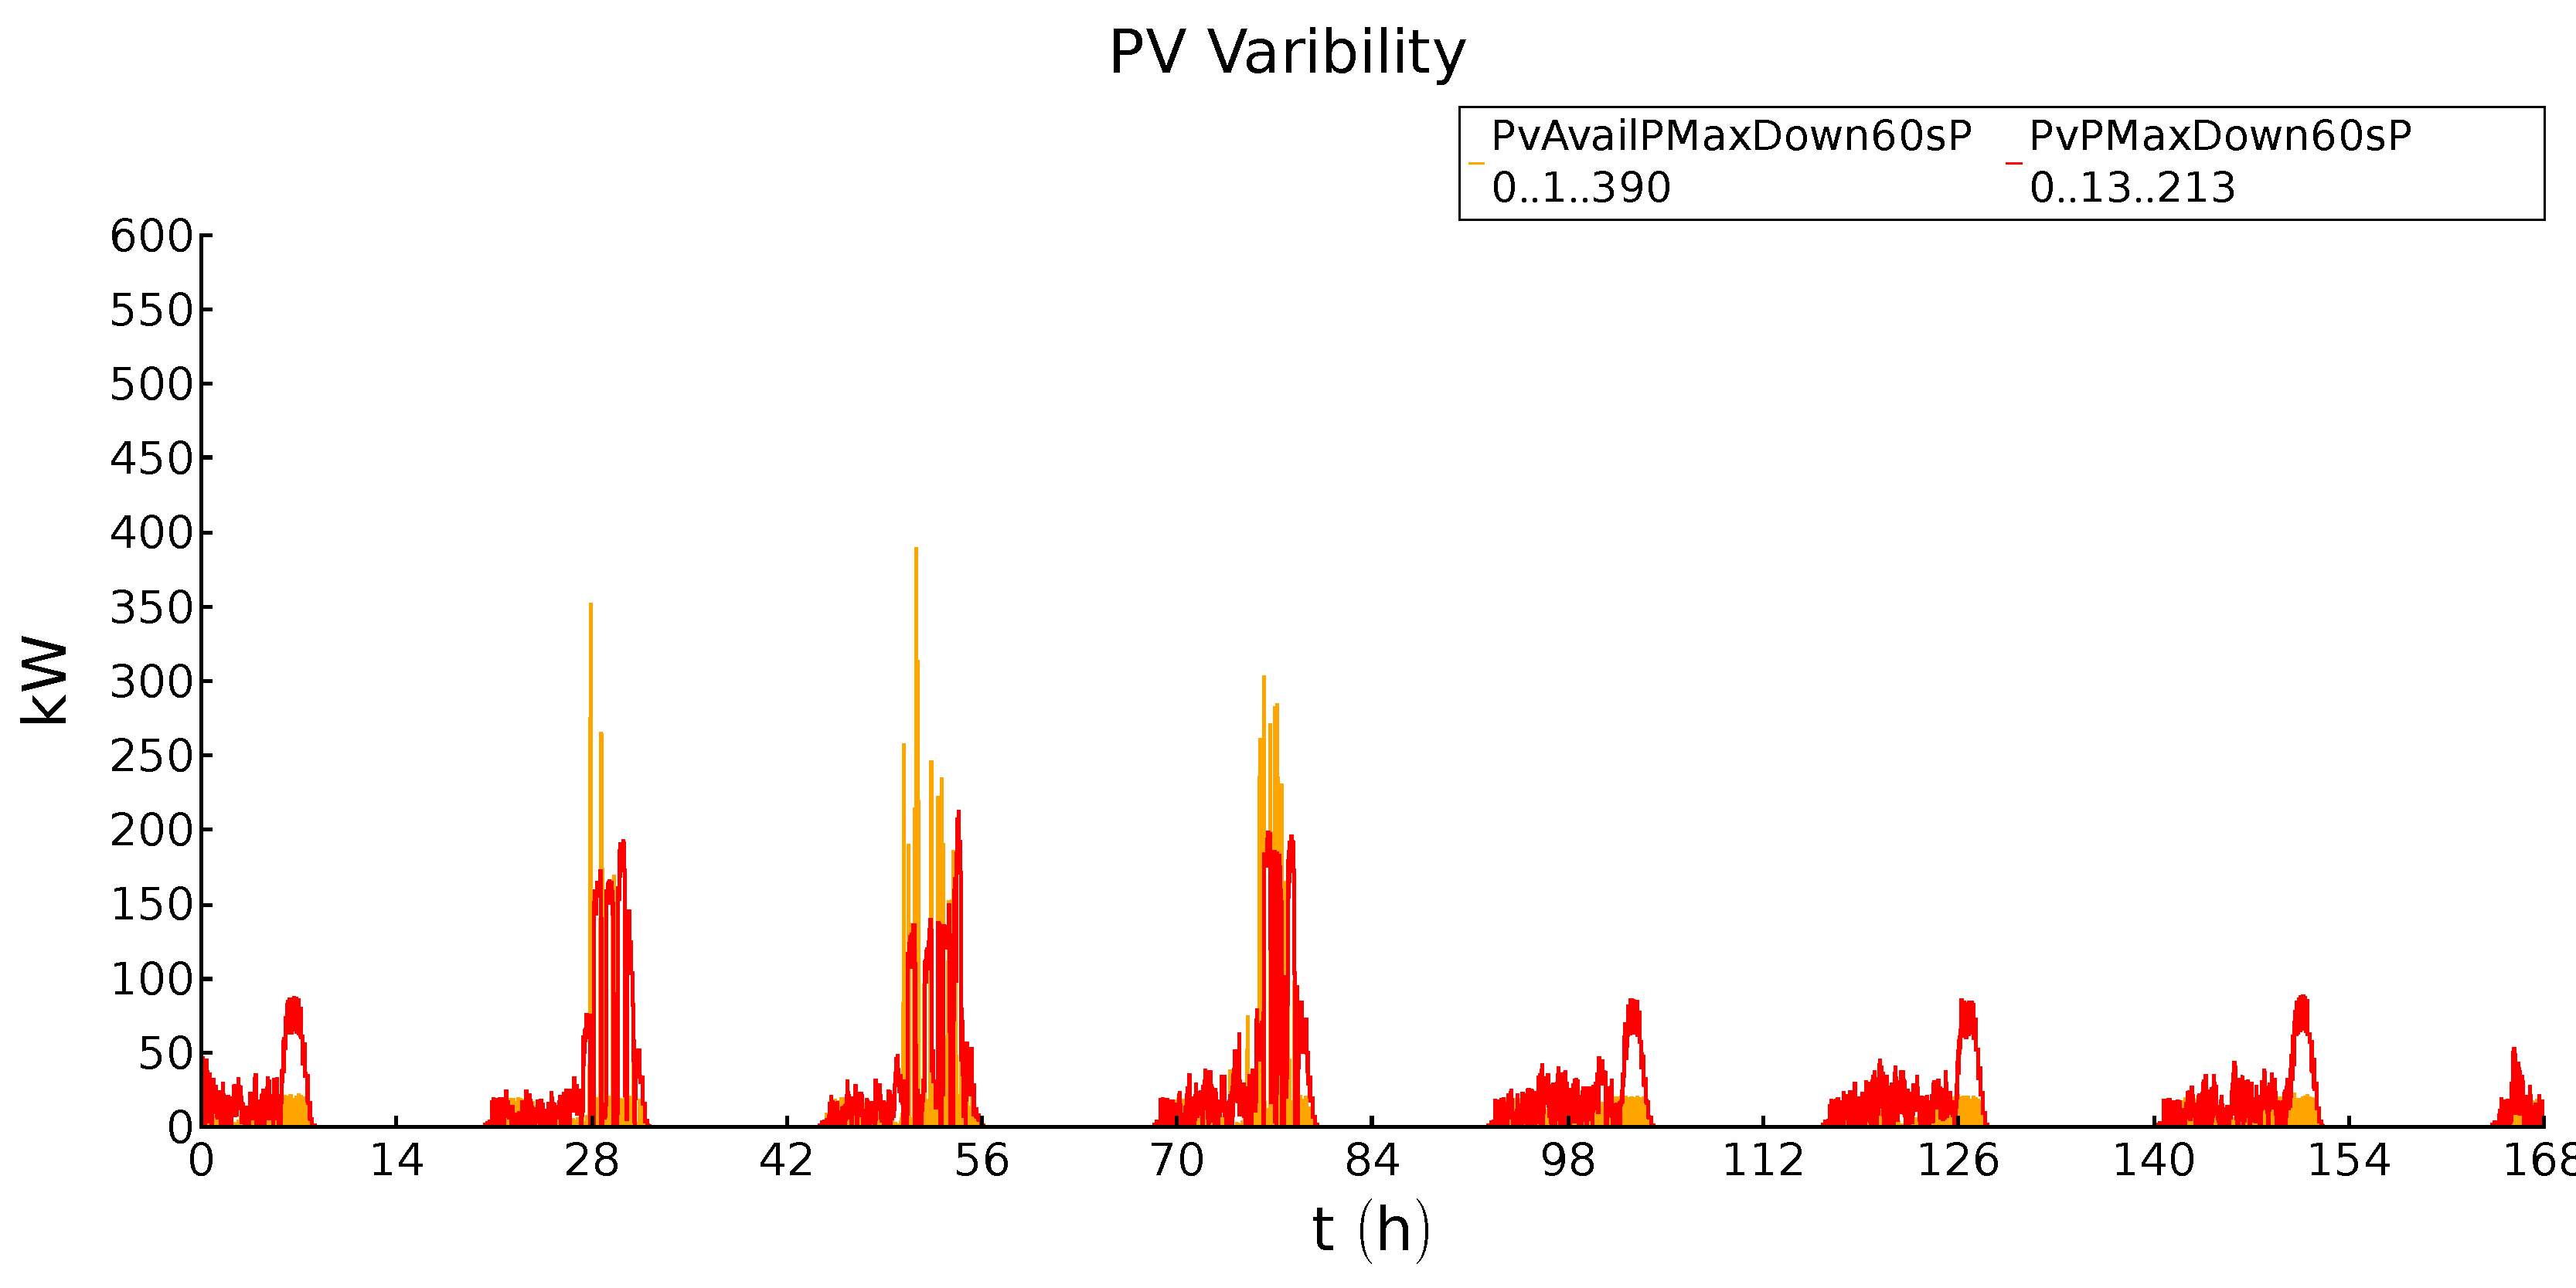
\includegraphics[width=9cm]{figPv2.pdf}  
\end{frame}

\section{Australia}
\begin{frame}\frametitle{ARENA}
  ARENA \href{www.arena.gov.au}{www.arena.gov.au} as approximately \$2.5 billion in funding to:
  \begin{enumerate}
  \item Fund renewable energy projects
  \item Support research and development activities
  \item Support activities to capture and share knowledge.
  \end{enumerate}
\pause
Projects larger than 26M\$:
\begin{itemize}
\item AGL Solar Project 166M\$
\item Australian Solar Thermal Research Initiative 35M\$
\item Australia-US Institute for Advanced Photovoltaics 33M\$
\item Cooper Basin Enhanced Geothermal Systems Heat/Power 59M\$
\item Kogan Creek Solar Boost project 34M\$
\item Moree Solar Farm 101M\$
\item NT SETuP Program 27M\$ (or 55M\$ total project)
\end{itemize}
\end{frame}

\begin{frame}\frametitle{Northern Territory: SETuP} 
  \begin{itemize}
  \item $>$30 sites medium penetration with 9MW PV and no storage.
    \pause
    Intended to reach 60\% peak penetration/contribution with a fuel
    saving of around 15\%.
  \item Single 1MW PV/Diesel/Battery site off (or 200\%
    penetration in Alaskan) with an intended fuel saving of around 50\%.
  \item Aiming to change the organisation and the technology.
  \end{itemize}
  \pause
  \begin{itemize}
  \item Sky Camera Forecasting
  \item Demand Management using Saturn South kit.
  \end{itemize}
  \pause
  Main point to note is that: 35 x anything is a lot, 35 x 2w for
  commissioning means a few years work.

  Contact: \href{mailto:andrew.gray@powerwater.com.au}{Andrew Gray}
\end{frame}

\section{Malaysia}
\begin{frame}\frametitle{Malaysia}
An overview of Malaysia.including 70\% average penetration, etc. ...
\end{frame}

\begin{frame}\frametitle{A wee system}
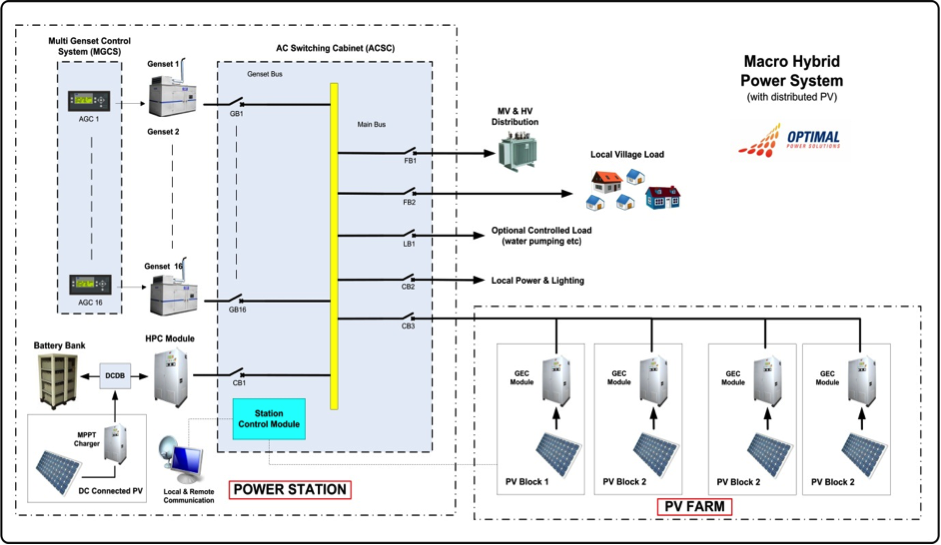
\includegraphics[width=9cm]{optimal_power_macro_hybrid_mini_grid_line_diagram_ops.png}
\end{frame}

\section{Sky Cameras}

\begin{frame}\frametitle{Sky Cameras}
Yet another modelfor procurement (for us at least:\footnote{Thanks to
  Tim Powe}).
  \begin{itemize}
  \item 3 x Trial Systems at a target price of 15k\$.for 3..6 months.
    \pause
  \item Everyone must provide a price for a:
    \begin{itemize}
    \item Trial system for 12 months.
    \item Rollout out of from 1..10 units over the next 2 years.
    \end{itemize}
  \end{itemize}
\end{frame}

\begin{frame}\frametitle{Sky Cameras: why}
Why we do it, who does it and how they do it.

All based on industrial input.
\end{frame}

\begin{frame}\frametitle{So who to talk to}
Who are the suppliers
\end{frame}

\section{Conclusion}
\begin{frame}\frametitle{Conclusion}
Nothing too controversial but:
\begin{itemize}
\item References to various projects.
\end{itemize}
\pause
\begin{quote}
``Economics are the method; 

\pause
the object is to change the heart and soul'' -- Margaret Thatcher
\end{quote}
\end{frame}
\end{document}

